\chapter{最终测试的补充结果}
\label{app:final-supplement}

本附录保留与第五章相同1200次留出测试对应的末段完整表、全程逐次分布和预先固定的空间快照，不新增运行，也不增加主要统计比较。每种方法与环境均包含30次独立运行。

\begin{table}[!htbp]
\centering\small
\caption{最终测试的末段合作均值与运行间标准差}
\label{tab:w2-final-tail}
\begin{tabular}{clrr}
\toprule
$r$ & 方法 & 干净 & 10\%持续失真 \\
\midrule
4.4 & 完整模型 & $0.97306\pm0.00020$ & $0.96852\pm0.00042$ \\
4.4 & 固定评分/学习门控 & $0.96866\pm0.00031$ & $0.96157\pm0.00039$ \\
4.4 & 学习评分/固定门控 & $0.95400\pm0.00032$ & $0.94302\pm0.00158$ \\
4.4 & 最高奖励/学习门控 & $0.96544\pm0.00034$ & $0.46601\pm0.02086$ \\
4.4 & 独立Q-learning & $0.38225\pm0.00061$ & $0.38225\pm0.00061$ \\
4.4 & 全局NI & $0.78733\pm0.31182$ & $0.03519\pm0.04733$ \\
4.4 & 局部NI & $0.37952\pm0.43339$ & $0.00544\pm0.00004$ \\
4.4 & 上尾过滤 & $0.03220\pm0.14723$ & $0.33912\pm0.38687$ \\
4.4 & 固定合作规则 & $0.92028\pm0.00015$ & $0.92076\pm0.00015$ \\
4.4 & 幅度校准固定规则 & $0.79391\pm0.00160$ & $0.70125\pm0.04456$ \\
\midrule
4.8 & 完整模型 & $0.98334\pm0.00007$ & $0.98443\pm0.00014$ \\
4.8 & 固定评分/学习门控 & $0.98549\pm0.00007$ & $0.98438\pm0.00012$ \\
4.8 & 学习评分/固定门控 & $0.97552\pm0.00007$ & $0.97443\pm0.00090$ \\
4.8 & 最高奖励/学习门控 & $0.98313\pm0.00014$ & $0.71329\pm0.01232$ \\
4.8 & 独立Q-learning & $0.45231\pm0.00248$ & $0.45231\pm0.00248$ \\
4.8 & 全局NI & $0.94500\pm0.00041$ & $0.12940\pm0.03935$ \\
4.8 & 局部NI & $0.72699\pm0.36598$ & $0.00553\pm0.00005$ \\
4.8 & 上尾过滤 & $0.89668\pm0.16831$ & $0.81964\pm0.01120$ \\
4.8 & 固定合作规则 & $0.94219\pm0.00008$ & $0.94238\pm0.00010$ \\
4.8 & 幅度校准固定规则 & $0.84281\pm0.00108$ & $0.83451\pm0.00102$ \\
\bottomrule
\end{tabular}
\par\smallskip{\zihao{-5}\rmfamily 来源：作者，本文冻结后的留出测试，每个条件30次独立运行，2026年。\par}
\end{table}


\begin{figure}[!htbp]
\centering
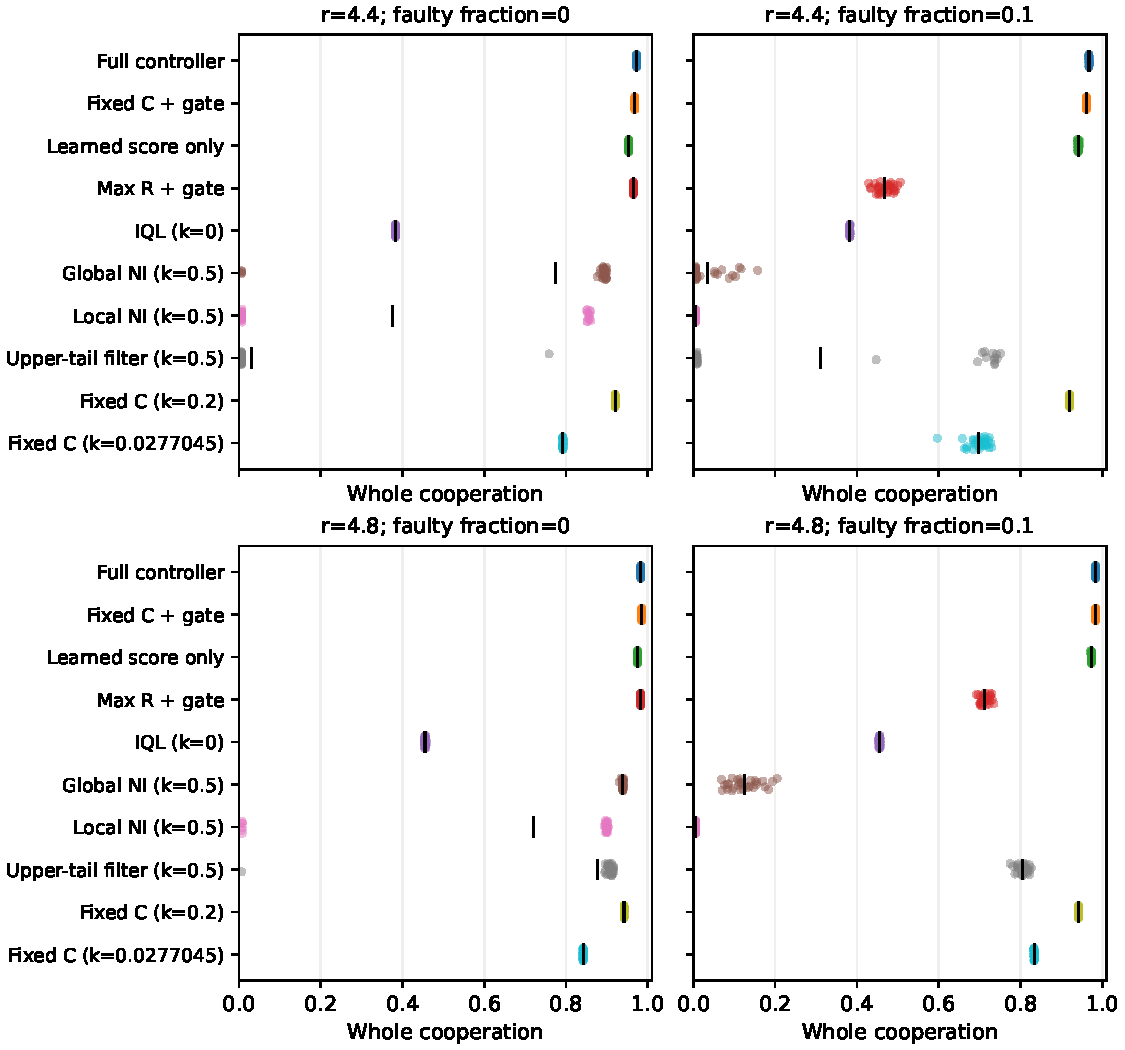
\includegraphics[width=\linewidth]{figures/work2-final/distributions-whole.pdf}
\caption{最终测试全部独立运行的全程合作。每个点对应一次100000步运行，黑色竖线为均值；纵向偏移仅用于分辨点。}
\label{fig:app-final-whole}
\par\smallskip{\zihao{-5}\rmfamily 来源：作者，本文冻结后的留出测试，每个条件30次独立运行，2026年。\par}
\end{figure}

\begin{figure}[!htbp]
\centering
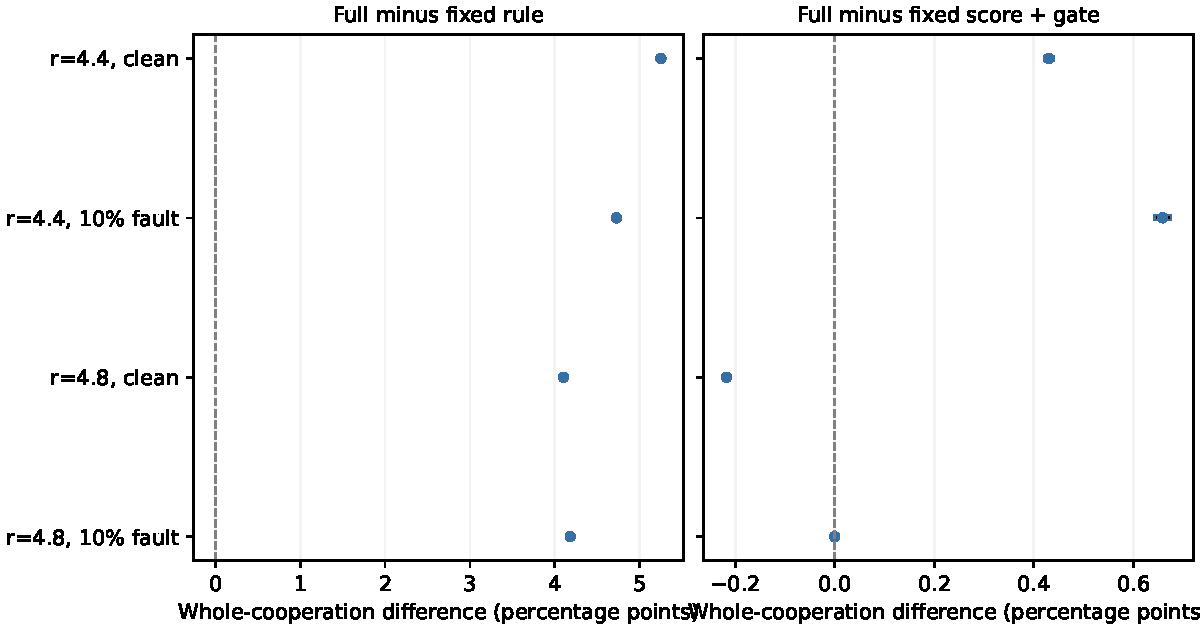
\includegraphics[width=\linewidth]{figures/work2-final/primary-differences.pdf}
\caption{八项主要比较的均值差与配对bootstrap区间。单位为百分点，差值方向为完整模型减去对照；黑色细线为95\%区间，蓝色粗线为对八项比较校正后的99.375\%近似区间。精确数值见表\ref{tab:w2-final-primary}。}
\label{fig:app-final-intervals}
\par\smallskip{\zihao{-5}\rmfamily 来源：作者，本文冻结后的留出测试，每个条件30次独立运行，2026年。\par}
\end{figure}

\begin{figure}[!htbp]
\centering
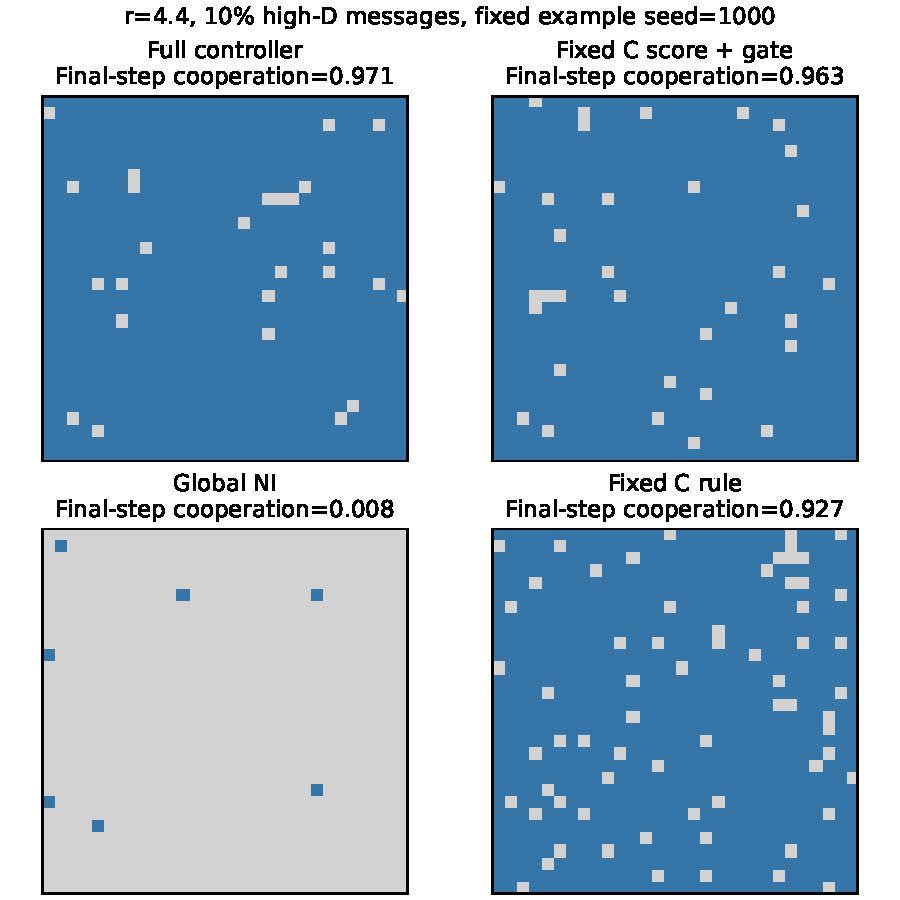
\includegraphics[width=.88\linewidth]{figures/work2-final/snapshots-r4.4.pdf}
\caption{最终测试中按同一预选规则取得的末轮真实动作，$r=4.4$、10\%持续失真。蓝色表示合作，灰色表示背叛；数值为末轮比例，与最后20\%窗口的均值不同。}
\label{fig:app-final-snapshot}
\par\smallskip{\zihao{-5}\rmfamily 来源：作者，本文冻结后的留出测试，每个条件30次独立运行，2026年。\par}
\end{figure}
